Linearized theory of Gravitational waves is a basic understanding of gravitational waves based on an assumption that any perturbation in space-time can be approximated to a linear factor whose degree is One. This simplifies the calculations a lot. And more over since the sources of gravitational waves are very far away, the effects they produce here on earth will be very small. So we can neglect the higher degree of perturbation and linearize it to the first degree. \\

Einstein's field equations are a set of ten Tensor equations which describe gravity as a curvature in space-time. And one among them is: 
\begin{equation}
    G_{\mu\nu}= \frac{8 \pi  G}{c^{4}}  T_{\mu\nu}
\end{equation}
This is a tensor equation which describes gravity in form of Einstein's tensor, $G_{\mu\nu}$ which is directly dependent on the geometry of space-time which is altered by the stress-energy tensor $T_{\mu\nu}$. Another field equation that relates the geometry or curvature of space-time to stress-energy tensor is 

\begin{equation}
    R_{\mu\nu}-\frac{1}{2}g_{\mu\nu}R=\frac{8\pi G}{c^{4}}T_{\mu\nu}
\end{equation}
where $R_{\mu\nu}$ is the Riemann tensor which describes the curvature of space-time, $R$ is the scalar curvature and $g_{\mu\nu}$ is the gravitational field tensor. Any change in matter distribution will be recorded in in $T_{\mu\nu}$. So if $T_{\mu\nu}$ changes then according to equation 2, gravitational field tensor $g_{\mu\nu}$ also has to change. If $h_{\mu\nu}$ is the perturbation induced in space-time then the new gravitational field tensor $\tilde{g}_{\mu\nu}$ is given by \cite{Kokkotas_2008}

\begin{equation}
    \tilde{g}_{\mu\nu} = g_{\mu\nu} + h_{\mu\nu}
\end{equation}

\noindent To get the new gravitational field, field equation should be solved for $\tilde{g}_{\mu\nu}$ which gives 

\begin{equation}
    \tilde{h}_{\mu\nu} = h_{\mu\nu} - \frac{1}{2} \, \eta_{\mu\nu} \, h^{\alpha}_{\alpha}
\end{equation}
 where $\eta_{\mu\nu}$ is the gravity where space is flat i.e. $\eta_{\mu\nu} = g_{\mu\nu}$ and $h^{\alpha}_{\alpha}$ is summed for all spatial coordinates i.e. $\alpha$ takes values $(1,2,3) $ which corresponds to $(x,y,z)$. The admitted solutions for this variations in space time $\tilde{h}_{\mu\nu}$ has solution in the form of 
 
 \begin{equation}
     \tilde{h}_{\mu\nu} = A^{\mu\nu}\, e^{ik_{\alpha}x^{\alpha}}
 \end{equation}
 
 \noindent This is a 3D wave equation where $A^{\mu\nu}$ is the Amplitude tensor, $i = \sqrt{-1} $, $k_{\alpha} = (k_{x},k_{y},k_{z})$ is the wave vector and $x^{\alpha} = (x^{1},x^{2},x^{2}) = (x,y,z)$ is the position vector.
 \\
 
 Thus we can say that when ever a body causes disturbances in curvature of space-time, these travel through space in form of waves whose speed is equal to the speed of light.  
 
\begin{figure}[h]
     \centering
     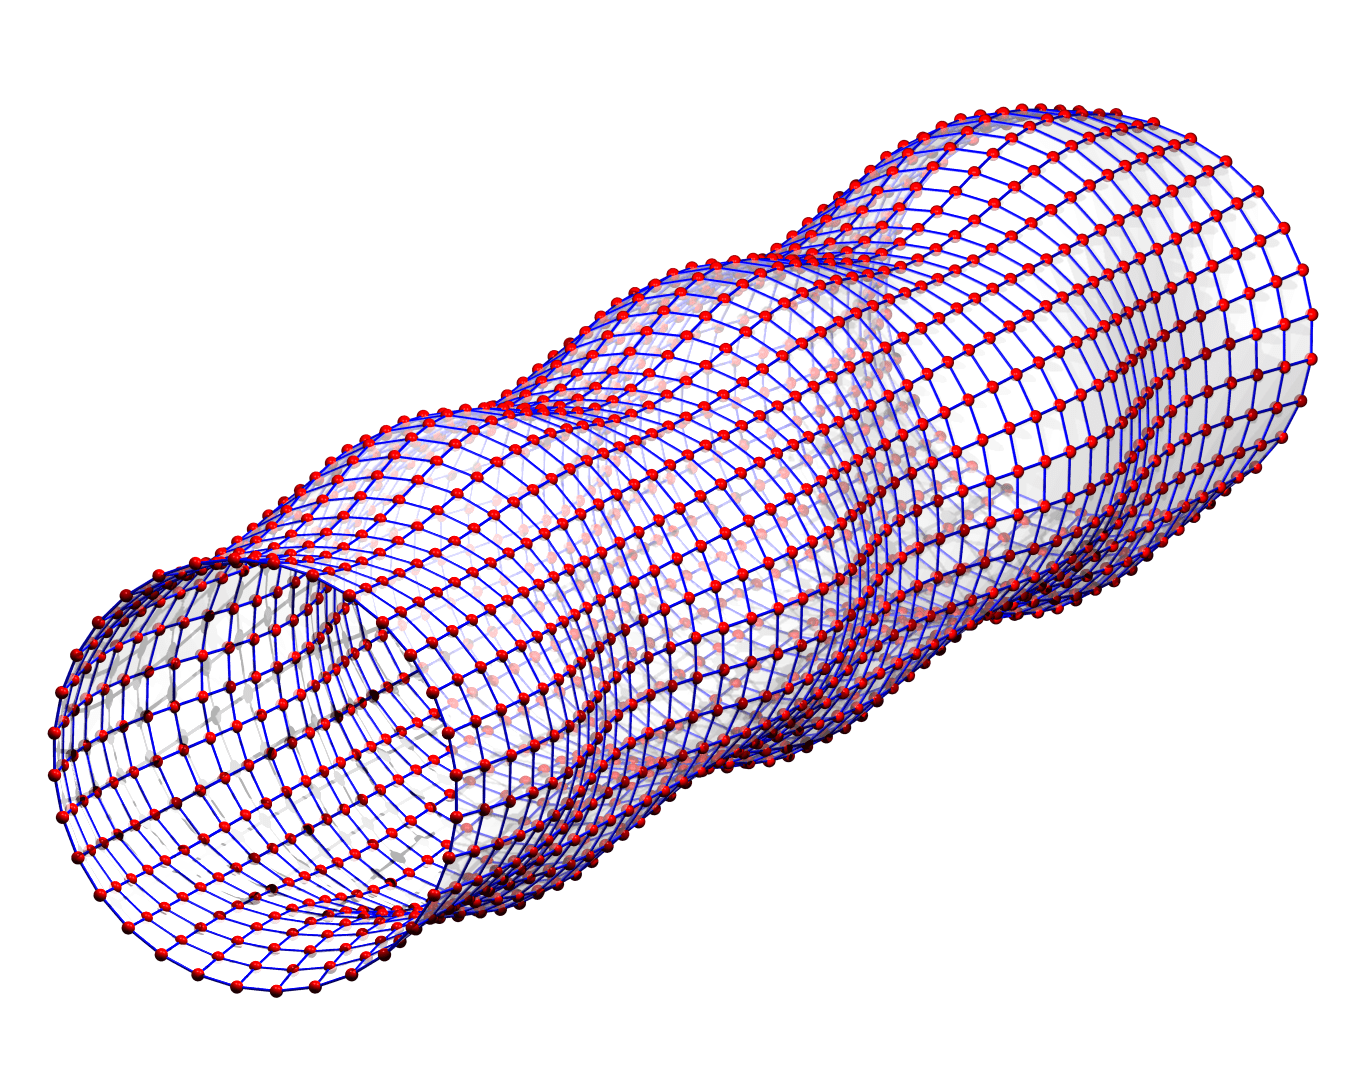
\includegraphics[scale=0.13]{images.tex/gw_representation.png}
     \caption{This is a computer simulated image that shows Gravitational wave as a 3D wave.\\ 
     Source:- \href{https://www.universetoday.com/127255/gravitational-waves-101/}{Universetoday.com}}
 \end{figure}
